\documentclass[12pt,a4paper]{article}

\usepackage[polish]{babel}
\usepackage[T1]{fontenc}
\usepackage[utf8]{inputenc}

\usepackage{geometry}
\geometry{margin=2.5cm}

\usepackage{graphicx}
\graphicspath{{img/}}

\usepackage{listings}
\lstset{
  basicstyle=\ttfamily\small,
  numbers=left,
  numberstyle=\tiny,
  stepnumber=1,
  frame=single,
}
\begin{document}

\begin{titlepage}
  \centering
  {\LARGE \textbf{Pierwszy dokument w LaTeX}\par}
  \vspace{1.5cm}
  {\large \textbf{Wstęp do Informatyki}\par}
  \vspace{1cm}
  \rule{\textwidth}{0.5pt}\par
  \vspace{0.8cm}
  {\large \textbf{Autorzy:}\par}
  {\large \textbf{Maciej Wrzesiński \\ Piotr Lik \\ Kacper Chrobak}\par}
  \vfill
  {\large \textbf{16.11.2025}\par}
\end{titlepage}

\tableofcontents
\newpage

\section{Maciej Wrzesiński}

\subsection{Wyrażenie matematyczne(jedynka trygonometryczna)}
\begin{equation}
  \sin^2 x + \cos^2 x = 1.
\end{equation}

\subsection{Grafika z podpisem}
\begin{figure}[h!]
  \centering
  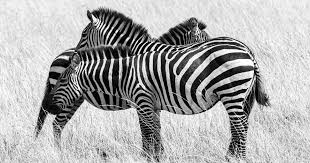
\includegraphics[width=0.7\linewidth]{image.png}
  \caption{Przykład iluzji optycznej}
\end{figure}

\subsection{Tabela trygonometryczna}
\begin{table}[h!]
  \centering
  \caption{Wartości funkcji sinus i cosinus dla wybranych kątów.}
  \begin{tabular}{|c|c|c|}
    \hline
    Kąt & $\sin \alpha$ & $\cos \alpha$ \\
    \hline
    $30^\circ$ & 0.5 & 0.87 \\ \hline
    $45^\circ$ & 0.71 & 0.71 \\ \hline
    $60^\circ$ & 0.87 & 0.5 \\
    \hline
  \end{tabular}
\end{table}


\subsection{Lista wypunktowana i numerowana}
\begin{itemize}
  \item punkt pierwszy,
  \item punkt drugi,
  \item punkt trzeci.
\end{itemize}

\begin{enumerate}
  \item krok 1
  \item krok 2
  \item krok 3
\end{enumerate}

\subsection{Fragment kodu}
\begin{lstlisting}
#include <stdio.h>

int sum(int *a, int n) {
    int s = 0;
    for (int i = 0; i < n; i++) s += a[i];
    return s;
}

int main(void) {
    int x[] = {1,2,3,4};
    printf("%d\n", sum(x, 4));
    return 0;
}
\end{lstlisting}

\subsection{Zainteresowania}

\hspace{0.65cm}Interesuję się ogólnie pojętą nauką w tym cyberbezpieczeństwem, dodatkowo historią XX wieku oraz geopolityką.

Lubię poszerzać swoje horyzonty. Studia są do tego idealną okazją.


\section{Piotr Lik}

\subsection{Fragment kodu (Assembler)}
\begin{lstlisting}
.intel_syntax noprefix
.global _start

.data
        my_message:
                .asciz "Hello, World!\n"
        message_len = . - my_message

.text
        _start:
                ;# sys_write
                mov rax, 1
                mov rdi, 1
                lea rsi, [rip + my_message]
                mov rdx, message_len
                syscall

                ;# sys_exit
                mov rax,60
                xor rdi, rdi
                syscall
\end{lstlisting}

\subsection{Matematyka}
Oto równanie kwadratowe w postaci ogólnej (bardzo popularne w matematyce)
\[a^2 + bx + c = 0\]
Do jego rozwiązania służy delta
\[\Delta = b^2 - 4ac\]
Gdy $\Delta = 0$ to rozwiązaniem jest
\[x = -\frac{b}{a}\]
A gdy $\Delta > 0$ to rozwiązaniamy są
\[x_1 = \frac{-b - \sqrt{\Delta}}{2a}\]
\[x_2 = \frac{-b + \sqrt{\Delta}}{2a}\]

\subsection{Grafika}
\begin{figure}[h!]
    \centering
    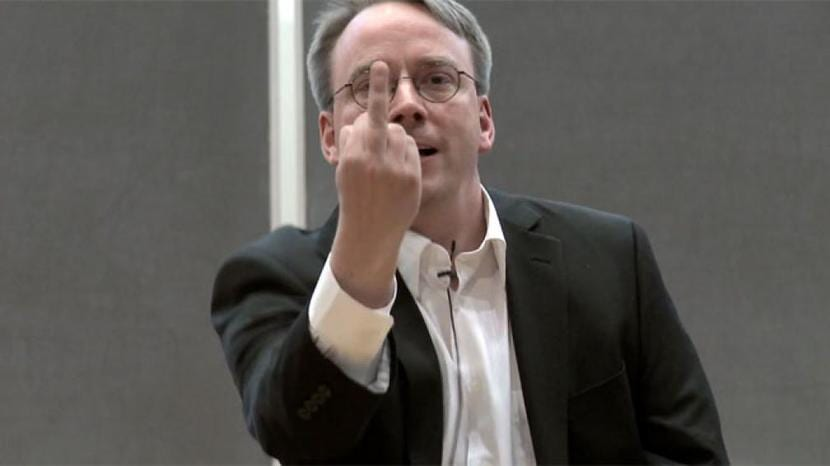
\includegraphics[width=0.7\linewidth]{linus.jpg}
    \caption{\textbf{Linus Torvalds} - fiński programista, twórca jądra \textit{Linux} oraz systemu kontroli wersji \textit{Git}}
\end{figure}

\newpage
\subsection{Tabliczka mnożenia}
\begin{table}[h!]
\centering
\begin{tabular}{|l|r|}
\hline
\textbf{Działanie} & \textbf{Wynik} \\
\hline
$9 \times 1$ & 9 \\
\hline
$9 \times 2$ & 18 \\
\hline
$9 \times 3$ & 27 \\
\hline
$9 \times 4$ & 36 \\
\hline
$9 \times 5$ & 45 \\
\hline
$9 \times 6$ & 54 \\
\hline
$9 \times 7$ & 63 \\
\hline
$9 \times 8$ & 72 \\
\hline
$9 \times 9$ & 81 \\
\hline
$9 \times 10$ & 90 \\
\hline
\end{tabular}
\caption{Tabliczka mnożenia liczby 9}
\end{table}

\subsection{Listy}
\begin{itemize}
    \item Element
    \item Inny element
\end{itemize}
\begin{enumerate}
    \item Pierwszy element
    \item Drugi element
\end{enumerate}

\subsection{O mnie}
\begin{abstract}
    \begin{center}
        Krótki opis moich zainteresowań
    \end{center}
\end{abstract}

Jestem studentem pierwszego roku cyberbezpieczeństwa, moimi zainteresowaniami jest architektura komputerów i programowanie w językach: \textit{C}, \textit{C++} i \textit{Python}

Z innych zainteresowań warto wymienić siłownię i \textit{Counter-Strike'a}

\section{Kacper Chrobak}
\subsection{Wzór matematyczny}
Tutaj wzór pitagorasa
\begin{center}
    $a^2 + b^2 = c^2$
\end{center}
\newpage
\subsection{Grafika kota}
\begin{figure}[h!]
  \centering
  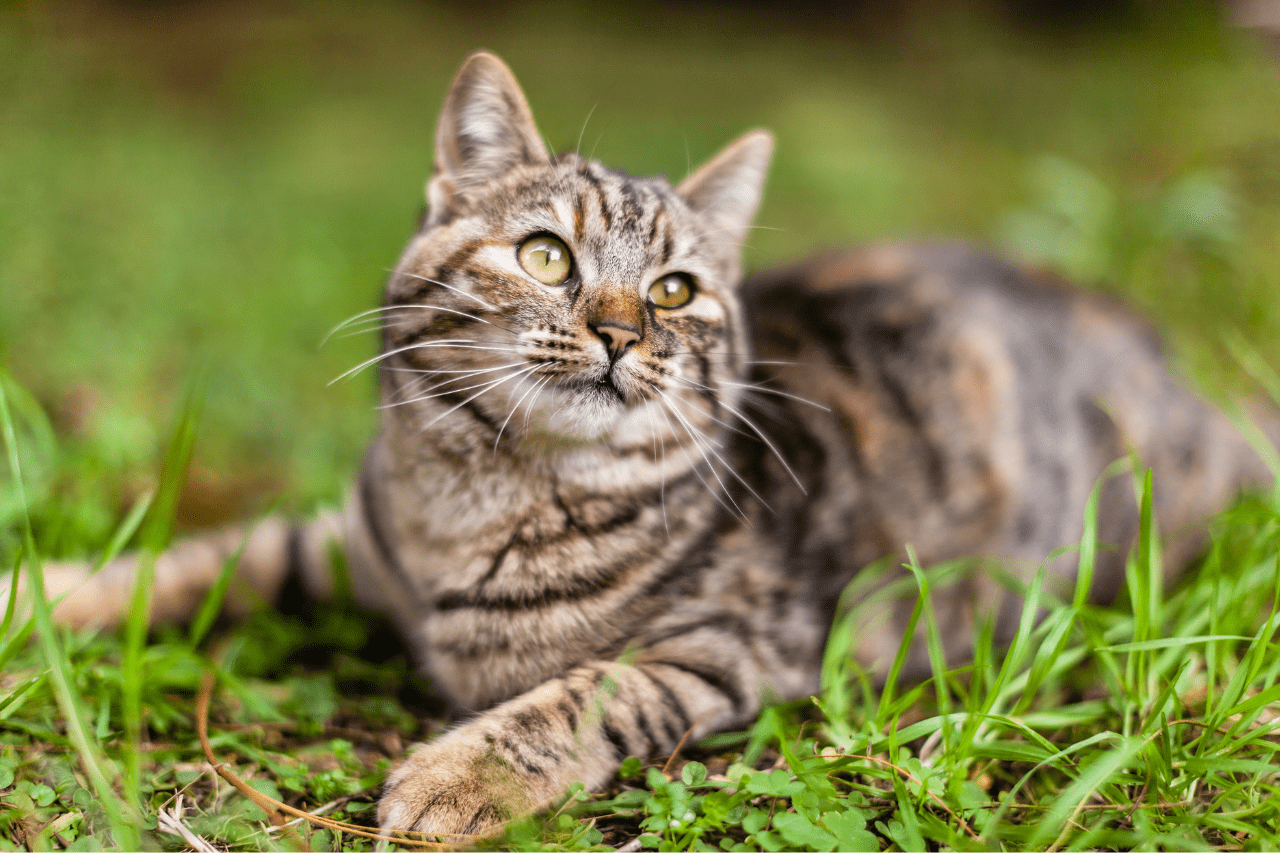
\includegraphics[width=0.5\linewidth]{img/Kot.png}
  \caption{Kotek}
\end{figure}
\subsection{tabela}
\begin{table}[h]
    \centering
    \caption{Tabela kilku funkcji logicznych}
    \renewcommand{\arraystretch}{1.2} % Troszkę więcej miejsca wierszach
    \begin{tabular}{|c|c|c|c|}
        \hline
        % --- Nagłówek (bez multirow) ---
        \textbf{Funkcja} & \multicolumn{3}{c|}{\textbf{Tabela}} \\ \cline{2-4}
        \textbf{logiczna} & \multicolumn{2}{c|}{Wejście} & Wyjście \\ \cline{2-4}
         & \textbf{p} & \textbf{q} & \textbf{s} \\ \hline

        % --- AND ---
        \textbf{AND} & 0 & 0 & 0 \\ \cline{2-4}
        % Pusta komórka po lewej daje efekt scalenia
         & 0 & 1 & 0 \\ \cline{2-4}
         & 1 & 0 & 0 \\ \cline{2-4}
         & 1 & 1 & 1 \\ \hline

        % --- OR ---
        \textbf{OR} & 0 & 0 & 0 \\ \cline{2-4}
         & 0 & 1 & 1 \\ \cline{2-4}
         & 1 & 0 & 1 \\ \cline{2-4}
         & 1 & 1 & 1 \\ \hline

        % --- NOT ---
        \textbf{NOT} & 0 & & 1 \\ \cline{2-4}
         & 1 & & 0 \\ \hline

    \end{tabular}
\end{table}
\subsection{lista}
\begin{itemize}
    \item to jest list wypunktowana
    \item a to jest drógi punkt
\end{itemize}
\begin{enumerate}
    \item a to jest lista numerowana
    \item i kolejny element tej listy
\end{enumerate}
\subsection{Fragment kodu}
\begin{lstlisting}
// Program ktory zawsze jest tworzony
#include <iostream>

int main() {
    std::cout << "Hello World!";
    return 0;
}
\end{lstlisting}
\subsection{Kacper Chrobak}
\begin{center}
    Jakie są moje zainteresowania?
\end{center}
Ogólnie rzecz biorąc interesuję się drukiem 3d, nową technologią, bezpieczeństwem w sieci, siecią internetową i majsterkowaniem. Jestem na studiach bo chciałem sie nauczyć nowych rzeczy
\end{document}

